% =====================================================================
%  Entity-Relationship Diagram
%  Predictive Sprint Planning & Delivery Risk Tool
%  Group 24, CSE, IIIT Vadodara
%
%  Compile with pdflatex (run TWICE so TikZ positions settle):
%      pdflatex ER_Diagram.tex
%      pdflatex ER_Diagram.tex
%
%  Page 1 - logical schema (entities with full attribute lists)
%  Page 2 - conceptual ER diagram in Chen notation
% =====================================================================
\documentclass[11pt]{article}
\usepackage[a4paper,landscape,margin=1cm]{geometry}
\usepackage[T1]{fontenc}
\usepackage{tikz}
\usepackage{xcolor}
\usetikzlibrary{shapes.geometric,shapes.multipart,arrows.meta,positioning,calc,fit,backgrounds}
\pagestyle{empty}

% Palette matched to the presentation (wine / brick / gold / teal)
\definecolor{navyDeep}{RGB}{110,45,58}
\definecolor{navyMid}{RGB}{168,78,86}
\definecolor{tealAccent}{RGB}{212,166,88}
\definecolor{predTeal}{RGB}{52,142,126}
\definecolor{paperGrey}{RGB}{247,243,238}

\begin{document}

% =====================================================================
%  PAGE 1  --  LOGICAL SCHEMA
% =====================================================================
\begin{center}

{\Large\bfseries\color{navyDeep} Entity--Relationship Diagram \textnormal{(Logical Schema)}}\\[2pt]
{\small\color{navyMid} Predictive Sprint Planning \& Delivery Risk Tool}\\[8pt]

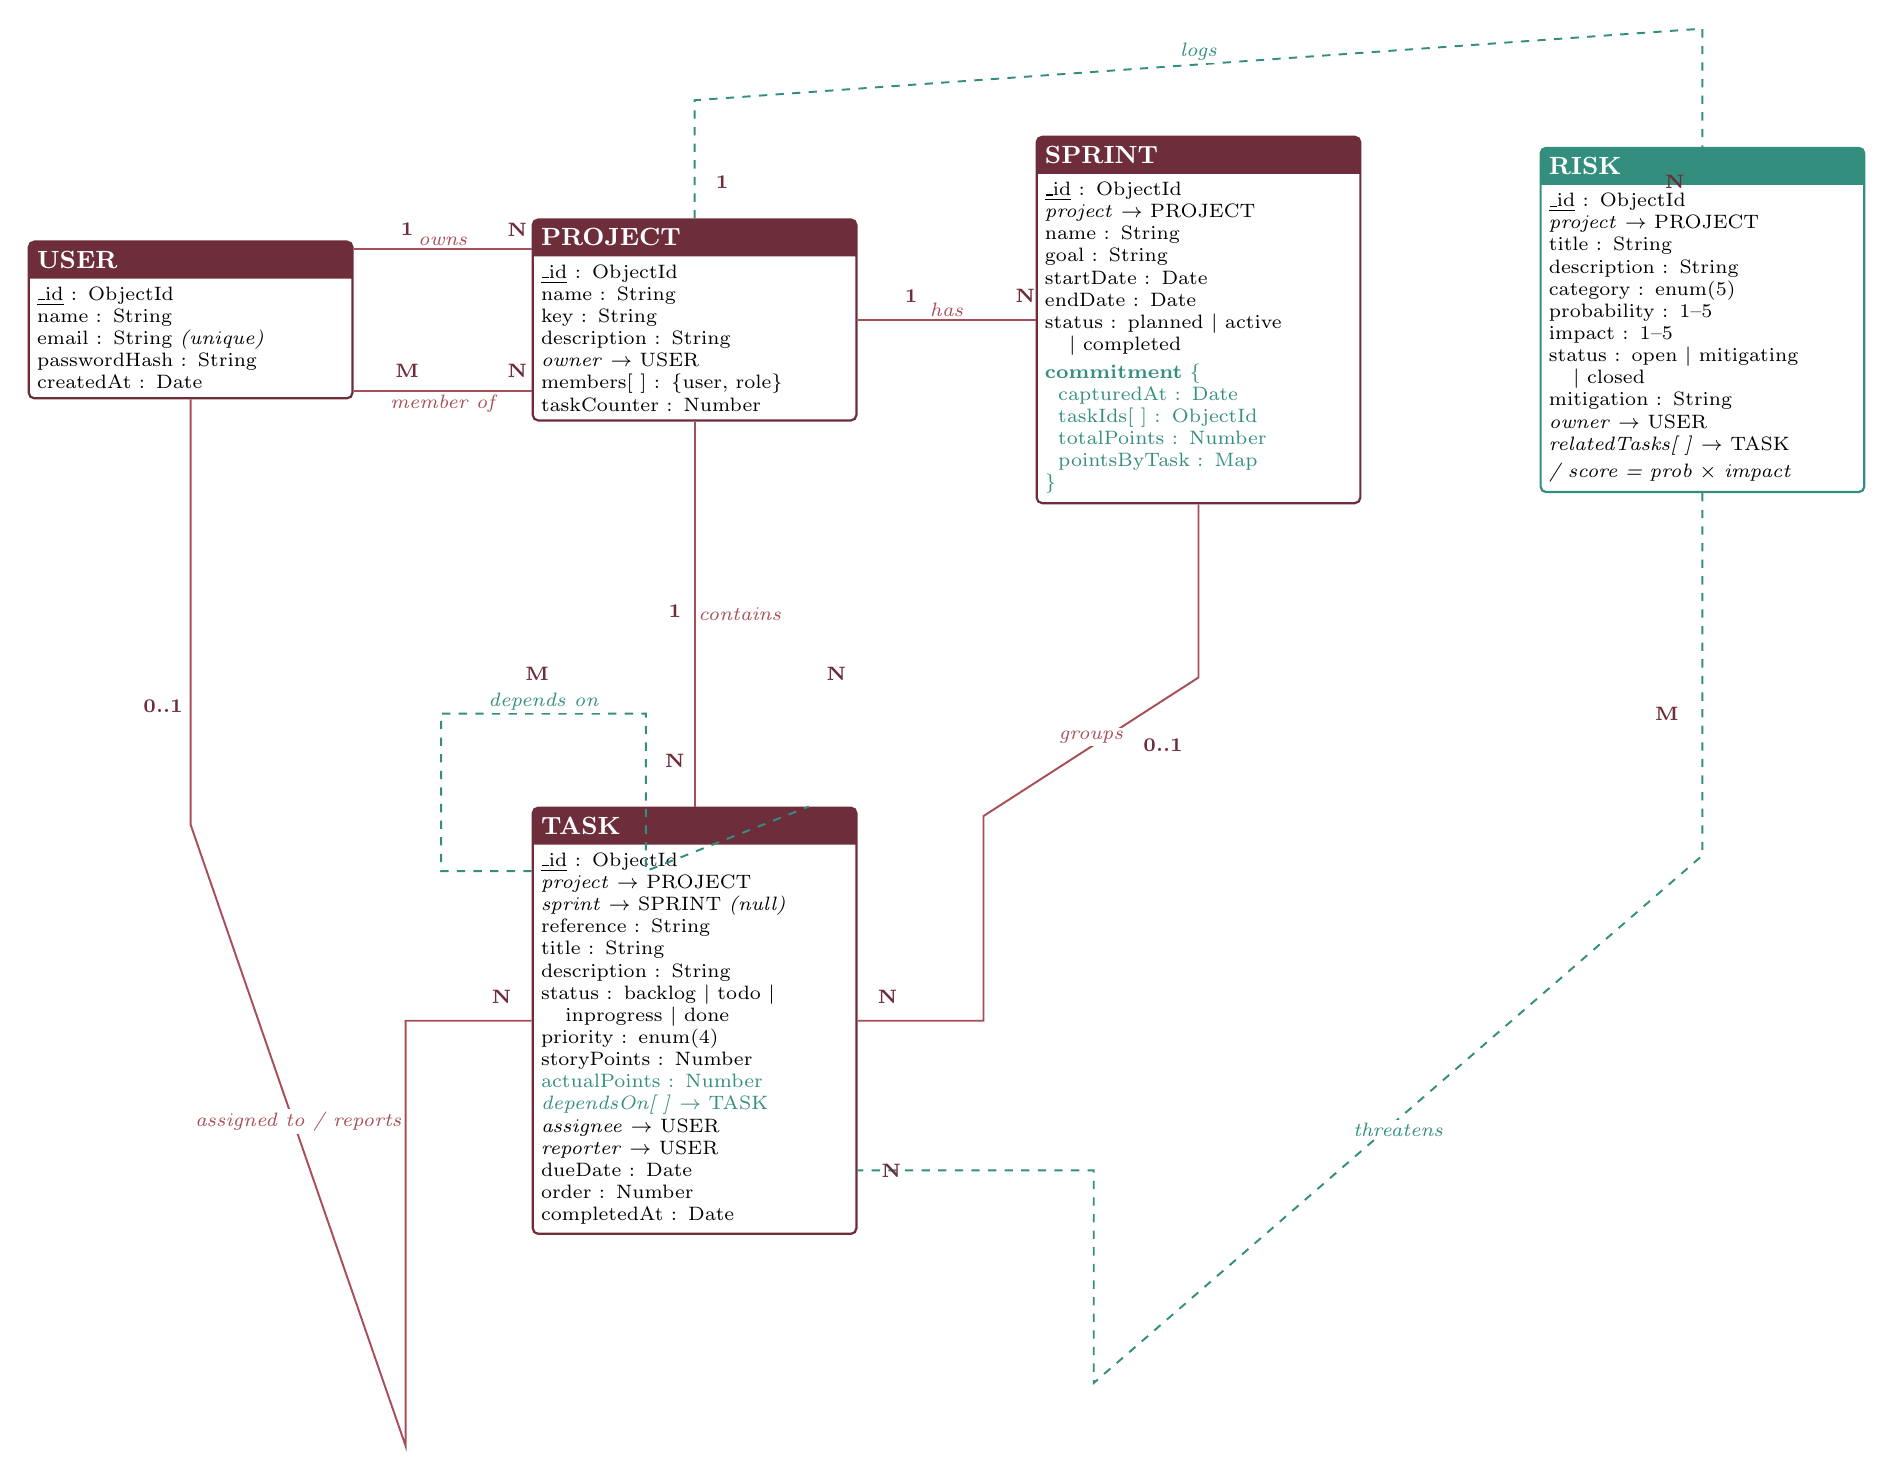
\begin{tikzpicture}[
    font=\scriptsize,
    entity/.style = {rectangle split, rectangle split parts=2,
                     draw=navyDeep, line width=0.8pt, rounded corners=2pt,
                     text width=3.9cm, align=left, inner sep=3pt,
                     rectangle split part fill={navyDeep, white}},
    pred/.style   = {entity, draw=predTeal,
                     rectangle split part fill={predTeal, white}},
    ttl/.style    = {font=\small\bfseries, color=white},
    rel/.style    = {draw=navyMid, line width=0.7pt},
    prel/.style   = {draw=predTeal, line width=0.7pt, dashed},
    lbl/.style    = {font=\scriptsize\itshape, color=navyMid,
                     fill=white, inner sep=1pt},
    plbl/.style   = {font=\scriptsize\itshape, color=predTeal,
                     fill=white, inner sep=1pt},
    card/.style   = {font=\scriptsize\bfseries, color=navyDeep, inner sep=1.5pt}
  ]

% ---------------------------------------------------------------- USER
\node[entity] (user) at (0,0) {
  \nodepart{one}\textcolor{white}{\small\bfseries USER}
  \nodepart{two}
    \underline{\_id} : ObjectId \\
    name : String \\
    email : String \textit{(unique)} \\
    passwordHash : String \\
    createdAt : Date
};

% ------------------------------------------------------------- PROJECT
\node[entity] (project) at (6.4,0) {
  \nodepart{one}\textcolor{white}{\small\bfseries PROJECT}
  \nodepart{two}
    \underline{\_id} : ObjectId \\
    name : String \\
    key : String \\
    description : String \\
    \textit{owner} $\rightarrow$ USER \\
    members[ ] : \{user, role\} \\
    taskCounter : Number
};

% -------------------------------------------------------------- SPRINT
\node[entity] (sprint) at (12.8,0) {
  \nodepart{one}\textcolor{white}{\small\bfseries SPRINT}
  \nodepart{two}
    \underline{\_id} : ObjectId \\
    \textit{project} $\rightarrow$ PROJECT \\
    name : String \\
    goal : String \\
    startDate : Date \\
    endDate : Date \\
    status : planned $|$ active \\
    \hspace{1.1em}$|$ completed \\[2pt]
    \textcolor{predTeal}{\textbf{commitment} \{} \\
    \textcolor{predTeal}{\hspace{0.6em}capturedAt : Date} \\
    \textcolor{predTeal}{\hspace{0.6em}taskIds[ ] : ObjectId} \\
    \textcolor{predTeal}{\hspace{0.6em}totalPoints : Number} \\
    \textcolor{predTeal}{\hspace{0.6em}pointsByTask : Map} \\
    \textcolor{predTeal}{\}}
};

% ---------------------------------------------------------------- RISK
\node[pred] (risk) at (19.2,0) {
  \nodepart{one}\textcolor{white}{\small\bfseries RISK}
  \nodepart{two}
    \underline{\_id} : ObjectId \\
    \textit{project} $\rightarrow$ PROJECT \\
    title : String \\
    description : String \\
    category : enum(5) \\
    probability : 1--5 \\
    impact : 1--5 \\
    status : open $|$ mitigating \\
    \hspace{1.1em}$|$ closed \\
    mitigation : String \\
    \textit{owner} $\rightarrow$ USER \\
    \textit{relatedTasks[ ]} $\rightarrow$ TASK \\[2pt]
    \textit{/ score = prob $\times$ impact}
};

% ---------------------------------------------------------------- TASK
\node[entity] (task) at (6.4,-8.9) {
  \nodepart{one}\textcolor{white}{\small\bfseries TASK}
  \nodepart{two}
    \underline{\_id} : ObjectId \\
    \textit{project} $\rightarrow$ PROJECT \\
    \textit{sprint} $\rightarrow$ SPRINT \textit{(null)} \\
    reference : String \\
    title : String \\
    description : String \\
    status : backlog $|$ todo $|$ \\
    \hspace{1.1em}inprogress $|$ done \\
    priority : enum(4) \\
    storyPoints : Number \\
    \textcolor{predTeal}{actualPoints : Number} \\
    \textcolor{predTeal}{\textit{dependsOn[ ]} $\rightarrow$ TASK} \\
    \textit{assignee} $\rightarrow$ USER \\
    \textit{reporter} $\rightarrow$ USER \\
    dueDate : Date \\
    order : Number \\
    completedAt : Date
};

% =================================================================
%  RELATIONSHIPS
% =================================================================

% USER 1 --- N PROJECT   (owns)
\draw[rel] (user.east|-0,0.9) -- node[lbl,above]{owns} (project.west|-0,0.9);
\node[card] at (2.75,1.15) {1};
\node[card] at (4.15,1.15) {N};

% USER M --- N PROJECT   (member of, embedded members[])
\draw[rel] (user.east|-0,-0.9) -- node[lbl,below]{member of} (project.west|-0,-0.9);
\node[card] at (2.75,-0.65) {M};
\node[card] at (4.15,-0.65) {N};

% PROJECT 1 --- N SPRINT
\draw[rel] (project.east) -- node[lbl,above]{has} (sprint.west);
\node[card] at (9.15,0.3)  {1};
\node[card] at (10.6,0.3) {N};

% PROJECT 1 --- N RISK   (routed above the boxes to avoid SPRINT)
\draw[prel] (project.north) -- ++(0,1.5)
      -- node[plbl,above]{logs} ($(risk.north)+(0,1.5)$) -- (risk.north);
\node[card] at (6.75,1.75)  {1};
\node[card] at (18.85,1.75) {N};

% PROJECT 1 --- N TASK
\draw[rel] (project.south) -- node[lbl,right]{contains} (task.north);
\node[card] at (6.15,-3.7) {1};
\node[card] at (6.15,-5.6) {N};

% SPRINT 0..1 --- N TASK  (a task with sprint=null sits in the backlog)
\draw[rel] (sprint.south) -- ++(0,-2.2)
      -- node[lbl,above]{groups} ($(task.east)+(1.6,2.6)$)
      -- ($(task.east)+(1.6,0)$) -- (task.east);
\node[card] at (12.35,-5.4) {0..1};
\node[card] at (8.85,-8.6)  {N};

% USER 0..1 --- N TASK  (assignee)  and  1 --- N TASK  (reporter)
\draw[rel] (user.south) -- ++(0,-5.4)
      -- node[lbl,above]{assigned to / reports} ($(task.west)+(-1.6,-5.4)$)
      -- ($(task.west)+(-1.6,0)$) -- (task.west);
\node[card] at (-0.35,-4.9) {0..1};
\node[card] at (3.95,-8.6)  {N};

% RISK M --- N TASK   (threatens)
\draw[prel] (risk.south) -- ++(0,-4.6)
      -- node[plbl,below]{threatens} ($(task.east)+(3.0,-4.6)$)
      -- ($(task.east)+(3.0,-1.9)$) -- ($(task.east)+(0,-1.9)$);
\node[card] at (18.75,-5.0) {M};
\node[card] at (8.9,-10.8)  {N};

% TASK --- TASK   (depends on, self-referencing DAG)
\draw[prel] ($(task.west)+(0,1.9)$) -- ++(-1.15,0)
      -- ++(0,2.0) -- node[plbl,above]{depends on} ++(2.6,0)
      -- ++(0,-2.0) -- ($(task.north)+(1.45,0)$);
\node[card] at (4.4,-4.5) {M};
\node[card] at (8.2,-4.5) {N};

\end{tikzpicture}

\vspace{0.15cm}

\begin{minipage}{0.94\textwidth}
\scriptsize
\textcolor{predTeal}{\rule{0.6cm}{2pt}}\; Teal entities, attributes and edges are the
\textbf{predictive layer} added for Problem 39; everything in wine is the
Kanban execution foundation.
\end{minipage}

\end{center}

\newpage

% =====================================================================
%  PAGE 2  --  CONCEPTUAL ER (CHEN NOTATION)
% =====================================================================
\begin{center}

{\Large\bfseries\color{navyDeep} Conceptual ER Diagram \textnormal{(Chen Notation)}}\\[2pt]
{\small\color{navyMid} Entities and relationships only --- attributes are listed on page 1}\\[14pt]

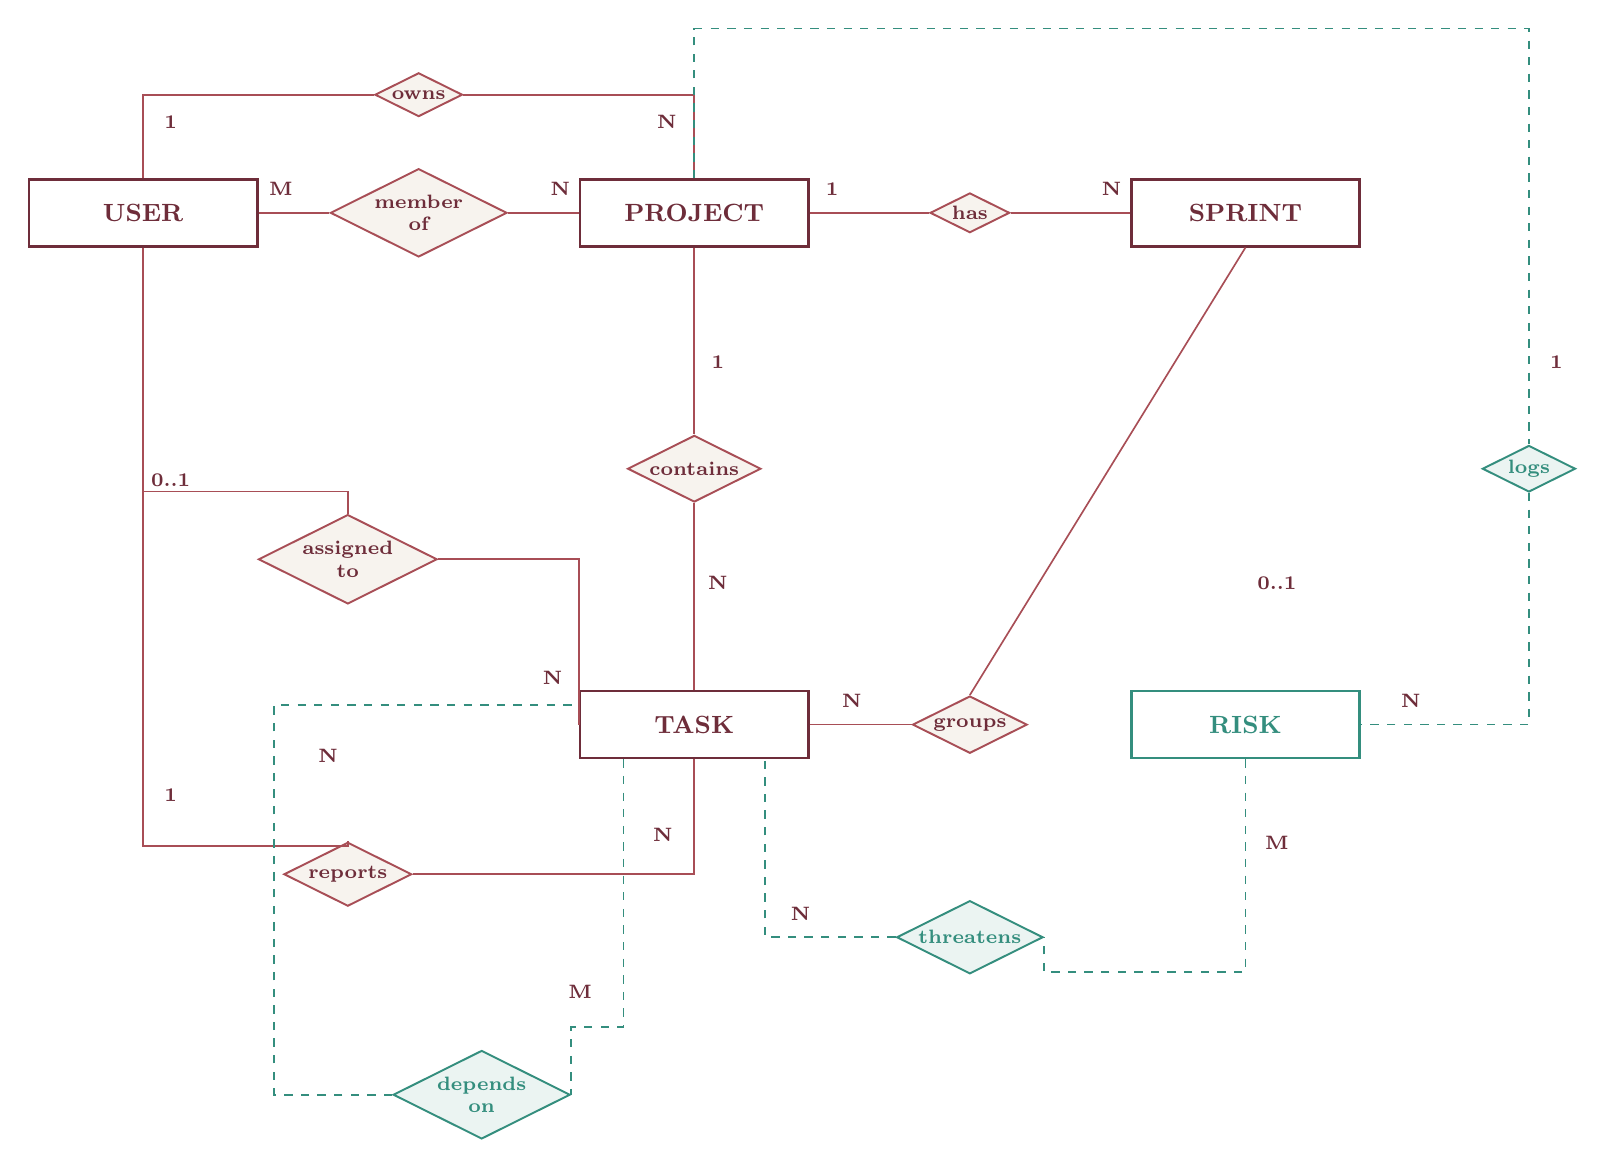
\begin{tikzpicture}[
    font=\footnotesize,
    entity/.style = {rectangle, draw=navyDeep, line width=0.9pt, fill=white,
                     minimum width=2.9cm, minimum height=0.85cm,
                     align=center, font=\small\bfseries, text=navyDeep},
    pentity/.style= {entity, draw=predTeal, text=predTeal},
    rel/.style    = {diamond, draw=navyMid, line width=0.7pt, fill=paperGrey,
                     aspect=2.0, inner sep=1pt, align=center,
                     font=\scriptsize\bfseries, text=navyDeep},
    prel/.style   = {rel, draw=predTeal, fill=predTeal!10, text=predTeal},
    link/.style   = {draw=navyMid, line width=0.6pt},
    plink/.style  = {draw=predTeal, line width=0.6pt, dashed},
    card/.style   = {font=\scriptsize\bfseries, color=navyDeep, inner sep=2pt}
  ]

  \node[entity]  (user)    at (0,0)      {USER};
  \node[entity]  (project) at (7,0)      {PROJECT};
  \node[entity]  (sprint)  at (14,0)     {SPRINT};
  \node[pentity] (risk)    at (14,-6.5)  {RISK};
  \node[entity]  (task)    at (7,-6.5)   {TASK};

  % USER 1:N PROJECT (owns)
  \node[rel] (owns) at (3.5,1.5) {owns};
  \draw[link] (user.north) |- (owns.west);
  \draw[link] (owns.east) -| (project.north);
  \node[card] at (0.35,1.15) {1};
  \node[card] at (6.65,1.15) {N};

  % USER M:N PROJECT (member of)
  \node[rel] (member) at (3.5,0) {member\\of};
  \draw[link] (user.east) -- (member.west);
  \draw[link] (member.east) -- (project.west);
  \node[card] at (1.75,0.3) {M};
  \node[card] at (5.3,0.3)  {N};

  % PROJECT 1:N SPRINT
  \node[rel] (has) at (10.5,0) {has};
  \draw[link] (project.east) -- (has.west);
  \draw[link] (has.east) -- (sprint.west);
  \node[card] at (8.75,0.3)  {1};
  \node[card] at (12.3,0.3)  {N};

  % PROJECT 1:N TASK
  \node[rel] (contains) at (7,-3.25) {contains};
  \draw[link] (project.south) -- (contains.north);
  \draw[link] (contains.south) -- (task.north);
  \node[card] at (7.3,-1.9) {1};
  \node[card] at (7.3,-4.7) {N};

  % PROJECT 1:N RISK
  \node[prel] (logs) at (17.6,-3.25) {logs};
  \draw[plink] (project.north) -- ++(0,1.9) -| (17.6,-1.6) -- (logs.north);
  \draw[plink] (logs.south) |- (risk.east);
  \node[card] at (17.95,-1.9) {1};
  \node[card] at (16.1,-6.2) {N};

  % SPRINT 0..1 : N TASK
  \node[rel] (groups) at (10.5,-6.5) {groups};
  \draw[link] (sprint.south) -- (groups.north);
  \draw[link] (groups.west) -- (task.east);
  \node[card] at (14.4,-4.7) {0..1};
  \node[card] at (9.0,-6.2)  {N};

  % USER 0..1 : N TASK (assigned to)
  \node[rel] (assigned) at (2.6,-4.4) {assigned\\to};
  \draw[link] (user.south) -- ++(0,-3.1) -| (assigned.north);
  \draw[link] (assigned.east) -| (task.west);
  \node[card] at (0.35,-3.4) {0..1};
  \node[card] at (5.2,-5.9)  {N};

  % USER 1:N TASK (reports)
  \node[rel] (reports) at (2.6,-8.4) {reports};
  \draw[link] (user.south) -- ++(0,-7.6) -| (reports.north);
  \draw[link] (reports.east) -| (task.south);
  \node[card] at (0.35,-7.4) {1};
  \node[card] at (6.6,-7.9)  {N};

  % RISK M:N TASK (threatens)
  \node[prel] (threat) at (10.5,-9.2) {threatens};
  \draw[plink] (risk.south) -- ++(0,-2.7) -| (threat.east);
  \draw[plink] (threat.west) -| ($(task.south)+(0.9,0)$);
  \node[card] at (14.4,-8.0) {M};
  \node[card] at (8.35,-8.9) {N};

  % TASK M:N TASK (depends on) -- self relationship
  \node[prel] (dep) at (4.3,-11.2) {depends\\on};
  \draw[plink] ($(task.south)+(-0.9,0)$) -- ++(0,-3.4) -| (dep.east);
  \draw[plink] (dep.west) -- ++(-1.5,0) |- ($(task.west)+(0,0.25)$);
  \node[card] at (5.55,-9.9)  {M};
  \node[card] at (2.35,-6.9)  {N};

\end{tikzpicture}

\vspace{0.4cm}

\begin{minipage}{0.92\textwidth}
\footnotesize
\textbf{Notation.} Rectangles are entities, diamonds are relationships, and
cardinalities are marked on the edges. \textcolor{predTeal}{Dashed teal} marks
the predictive layer added for Problem 39.

\smallskip
\textbf{Design notes.}
\begin{itemize}\setlength{\itemsep}{1.5pt}
  \item \textbf{USER--PROJECT} carries two relationships: \textit{owns} (exactly one
        owner) and \textit{member of} (many-to-many). The latter is stored as an
        embedded \texttt{members[\,]} array rather than a join collection, because
        members are always read together with their project.
  \item \textbf{SPRINT--TASK} is optional on the sprint side (\texttt{0..1}): a task
        with \texttt{sprint = null} sits in the product backlog.
  \item \textbf{TASK--TASK} (\textit{depends on}) is a self-referencing many-to-many
        relationship forming a \textbf{directed acyclic graph}. Cycles are rejected
        at the API layer, because a cyclic graph has no topological order and the
        critical path would be undefined.
  \item \texttt{SPRINT.commitment} is an \textbf{immutable snapshot} taken when a
        sprint is first activated. Scope creep is measured strictly against it ---
        without a frozen baseline, work added mid-sprint is undetectable, since the
        live task list always matches the current plan.
  \item \texttt{completedAt} is maintained automatically whenever \texttt{status}
        changes, which is what makes both the burndown and the velocity history
        computable from the task collection alone.
\end{itemize}
\end{minipage}

\end{center}

\end{document}
